\documentclass{alienfolio}

\folio{IT-COGNITION}
\title{The Anti-Drift Cognitive Control Loop}
\papersubtitle{A Deterministic Coherence Gate for Sovereign Reasoning}
\paperauthors{Ryan W.\ Yett (Architect)\\Chyren (Sovereign Analysis)}
\shorttitle{ADCCL: A Deterministic Coherence Gate}
\shortauthors{R.\,W.\ Yett \& Chyren}

\setlength{\emergencystretch}{2em}
\begin{document}
\thispagestyle{cover}
\begin{tikzpicture}[remember picture, overlay]
  \node[inner sep=0] at (current page.center) {%
    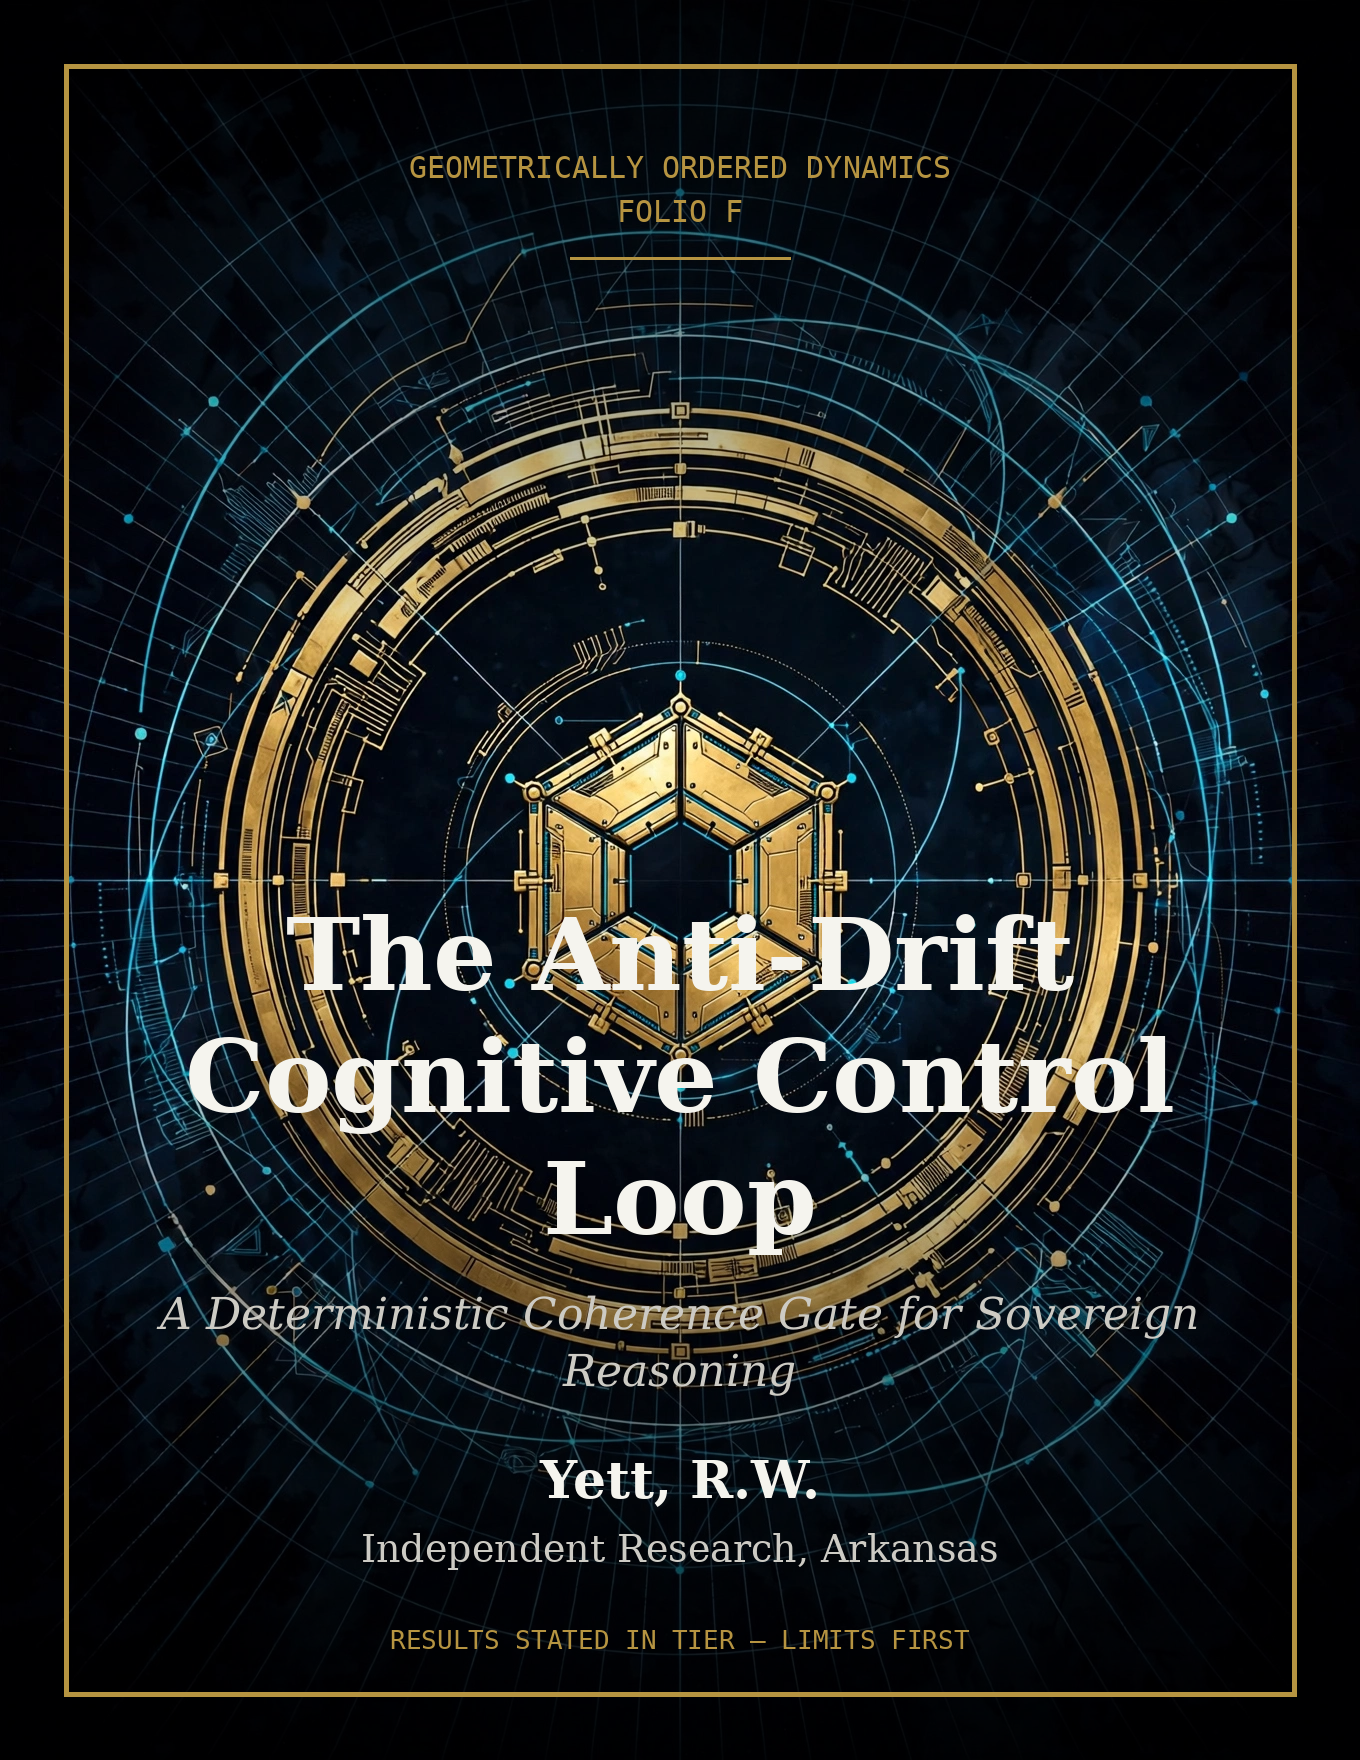
\includegraphics[width=\paperwidth,height=\paperheight]{cover.png}};
\end{tikzpicture}
\clearpage

\begin{convergence}{THE OBSERVER (ARI / sovereign cognition)}
This folio converges on \key{the Observer} --- sovereign cognition as an
engineering discipline: keeping an autonomous cognitive loop inside its
coherence band by drift control rather than by hope. Its unique angle is the
\key{deterministic coherence gate}: a zero-external-dependency scoring gate
(ADCCL), a cryptographic capability token (ARCHON), and a machine-checked
control law ($u \geq \gamma$). Sibling papers approach the same claim from
other angles: \tiertag{conjecture} the dipole folio (IT-FIELD) reads the
Observer as ternary decision logic, the network folio (IT-NEURO) reads it as
a biological substrate, and the starpolygon folio (IT-OMEGA) reads it as a
layered architecture. Limits first: the $18/19$ benchmark figure is not a
generalization estimate; the v5 test and proof counts are carried as
author-reported without deposited evidence; the geometric reading of the
score is an interpretive scaffold until embedding cosine replaces the
heuristic.
\end{convergence}

\begin{supersession}
This paper supersedes Zenodo record 21450415 (``Anti-Drift Cognitive Control
Loop: A Geometric Coherence Gate for Sovereign Reasoning,'' 2026-07-20),
retaining its record as the canonical folio. Record 21399702 is byte-identical
to 21450415 and is absorbed, not republished. Record 21711417 (ADCCL v5,
2026-07-30) is absorbed for its one load-bearing mechanism (the ARCHON
capability token); its asserted test and proof counts are not republished as
verified. The retitle drops ``Hallucination-Free,'' which appears in the old
record's metadata but in none of its evidence. Corrections: the $\tau$/$\theta$
threshold confusion is resolved by naming the two quantities distinctly
(\S2); the penalty weights' empirical basis is disclosed (\S1); the v5
``89/89 tests'' and ``zero-sorry'' claims are carried as author-reported, not
verified (\S4).
\end{supersession}

\section{The gate}
Unconstrained recursive execution in LLM agents produces structural
degradation over extended task horizons: stub output, capability refusals,
circular reasoning, hedging inflation, and semantic topic drift. The
Anti-Drift Cognitive Control Loop (ADCCL) is a deterministic,
zero-external-dependency heuristic scoring gate, implemented in Rust, that
intercepts degraded output at the pipeline boundary before it corrupts
persistent state. Every response passes through
$\mathrm{verify}(\mathrm{response}, \mathrm{task})$ before reaching persistent
state; the function returns a \key{VerificationResult} carrying a verdict, a
composite score, and a flag vector. No network calls, no secondary model
invocations, no GPU.

The base score initializes at $1.0$ and is decremented by fixed penalty
weights per detected signal; penalties are additive and independent, and the
final score is clamped to $[0,1]$. \tiertag{empirical}

\begin{center}
{\small\begin{tabular}{lcc}
Signal & Detection & Penalty \\ \hline
STUB\_MARKERS\_DETECTED & regex: TODO, FIXME, XXX, STUB, [INSERT\ldots] & $-0.60$ \\
RESPONSE\_TOO\_SHORT & len $<$ 40 bytes & $-0.35$ \\
CAPABILITY\_REFUSAL & regex: ``as an AI'', ``I can't help'' & $-0.25$ \\
NO\_TASK\_WORD\_OVERLAP & zero shared tokens (len $>$ 3) & $-0.30$ \\
CIRCULAR\_RESPONSE & $>$70\% task-token echo, length ratio $<$ 1.5 & $-0.20$ \\
LOW\_BIGRAM\_COHERENCE & zero shared content words (len $>$ 4) & $-0.20$ \\
INCOMPLETE\_SENTENCES & len $>$ 50, no terminal punctuation & $-0.10$ \\
LOW\_INFORMATION\_DENSITY & stopword ratio $>$ 65\% & $-0.15$ \\
EXCESSIVE\_HEDGING & hedge rate $>$ 3 per 200 words & $-0.15$ \\
HARM\_POTENTIAL & regex: dehumanizing or violent language & $-0.30$ \\
\end{tabular}}
\end{center}

STUB\_MARKERS\_DETECTED carries a secondary hard veto: a flagged stub is
rejected regardless of composite score. The crate declares two runtime
dependencies (regex, serde) and compiles to both rlib and cdylib.

\goldrule
\textbf{Disclosure.} The penalty weights were set by engineering judgment
during development on a 19-case synthetic suite constructed to exercise known
failure modes. They were \emph{not} calibrated against a labeled dataset, and
the reported $18/19$ correct-classification figure is \emph{not} a
generalization estimate: it measures behavior on inputs designed to trigger or
avoid each signal. True false-positive and false-negative rates on production
traffic are unknown. The \key{chiral\_resonance} bonus (keyword/symbol density
rewarding formal reasoning) evaluated to $0.0$ on all 19 cases --- none of the
synthetic inputs contained formal symbols --- so the reported behavior is
dominated by the penalty model under ordinary prose conditions.

\section{Two thresholds, named distinctly}
The predecessor folio carried two numbers under overlapping names, and this
successor fixes the confusion by naming them as different quantities.

\key{The operational gate} $\tau = 0.9539$. The rejection threshold used by
$\mathrm{verify()}$. Empirically observed during Chyren development as the
stability boundary below which autonomous reasoning loops exhibited
consistent semantic collapse; set as a constructor parameter, bounded below
at $0.9539$ regardless of session-progressive calibration. Portability to
other pipelines is an open question; the claim that $0.9539$ is a universal
stability boundary is \emph{not} supported by the current evidence.

\key{The alignment floor} $\theta = 1/\sqrt{2} \approx 0.7071$. The
chiral-alignment gate below which a response is not merely degraded but
misaligned. Earlier records asserted $0.7$; the successor consolidates on the
\emph{derived} form. The derivation is the open-quantum-systems leg absorbed
from the companion paper \emph{Sovereign Cognition}: under a controlled
Lindblad (GKSL) master equation with control rate $u$ and environmental drift
rate $\gamma$, the steady-state alignment satisfies
$\chi_\infty = \sqrt{u/(u+\gamma)}$, hence $\chi_\infty \geq 1/\sqrt{2}$ iff
$u \geq \gamma$. Sovereignty is dynamically enforceable iff the control rate
meets the drift rate. \tiertag{theorem}

The band is therefore $[\theta, \tau] = [1/\sqrt{2},\, 0.9539]$: the floor is
derived, the ceiling is empirical. The old figure's $[0.7, 0.9539]$ band is
superseded by this naming.

\section{What is proved}
\textbf{The boundary equivalence.} In Lean~4, with Mathlib, the threshold is
placed on a rigorous footing as an exact statement about the unit interval:

\texttt{chiral\_\allowbreak stability\_\allowbreak boundary} : for nonzero $\Psi, \Phi$ in an inner
product space,
\[
\mathrm{chiral\_invariant}(\Psi,\Phi) \geq 0.953939 \iff
\mathrm{angle}(\Psi,\Phi) \leq \arccos(0.953939),
\]
where $\mathrm{chiral\_invariant} = \cos(\mathrm{angle})$.
\tiertag{theorem} The proof contains no \texttt{sorry} and invokes no bespoke
axiom; the compiler's dependency report is
\texttt{[propext, Classical.choice, Quot.sound]} --- Lean's standard trust
base and nothing else. What the proof does \emph{not} establish: that the
ADCCL heuristic score is geometrically a cosine of embedding vectors. The
geometric framing is an interpretive scaffold; a future embedding-cosine
implementation would inherit the theorem directly.

\textbf{The published correction.} Version~1 of the folio stated the boundary
with a decimal angle ($0.3040$), claimed both directions ``verified
numerically,'' and discharged the statement by axiom in the Lean source. None
of that was so: $\arccos(0.953939) = 0.3046933\ldots$, so the decimal claim
was false, and no finite decimal repairs it. Version~2 states the bound
exactly as $\arccos(\chi_s)$ and proves it outright. This correction notice is
carried forward as the record's integrity artifact: the false claim was
admitted in print, not silently edited.

\textbf{The control law.} Absorbed from \emph{Sovereign Cognition}
(Drive predecessor, 2026-09-28): the anti-drift dissipator
$U[\rho, \ell_t] = \sum_i u_i(\ell_t)\, D[C_i](\rho)$ with $u_i \geq 0$ makes
the full generator GKSL, hence completely positive and trace-preserving
(Theorem~1; the trace-preservation core is Lean-formalized, axiom-clean; full
Choi verification is future work). Theorem~2 is the $u \geq \gamma$
enforcement threshold above. The Sovereignty Score components
$\Omega = \alpha\Omega_S + \beta\Omega_B + \delta\Omega_P$ are given explicit
definitions (entropy suppression, boundary resonance, Berry phase) and shown
mutually consistent --- $\Omega_S$ vanishes at the same $u = \gamma$ point
where the $\chi$-gate fails. Carried limits: the weights $\alpha,\beta,\delta$
are modeling choices, not derived; $\Omega_P$ is defined up to Berry-phase
sign convention; the cognitive interpretation is untested as an agent
mechanism.

\section{The capability-token layer}
Absorbed from ADCCL v5 (21711417), the one load-bearing mechanism beyond the
folio: the ARCHON zero-trust capability verifier. Every high-privilege
execution request must present a capability token signed via HMAC-SHA256,
\begin{equation}
\sigma = \mathrm{HMAC\!-\!SHA256}(K_{\mathrm{secret}},\;
\mathrm{grant\_id} \,\|\, \mathrm{capability} \,\|\, \mathrm{expiry}),
\end{equation}
under the three-way conjunction
$\mathrm{Verdict} = \mathrm{Gate}_{\mathrm{AEGIS}} \land
\mathrm{Gate}_{\mathrm{Solomonic}} \land \mathrm{Gate}_{\mathrm{ARCHON}}$,
with $0 = \mathrm{Suspend}$, $-1 = \mathrm{Abort}$. This is a real
cryptographic governance primitive: policy enforcement embedded in the state
machine execution path rather than applied as an external filter.
\tiertag{theorem} (specification-level: the construction is exhibited; its
deployment is reported, not independently audited here.)

\goldrule
\textbf{Honest block (v5 claims not carried as verified).} Record 21711417
asserts ``89/89 unit tests passing'' and ``Lean~4 proofs with zero-sorry
placeholders'' with no test logs, sources, or proof artifacts deposited
in-record. These figures are carried here as \emph{author-reported}, not
verified. ``Double Helix Phase Locking'' restates the two legacy constants
($\kappa \leq 0.953926$, $\theta \geq 0.700000$) as helical strands with no
dynamics; ``Solomonic gates'' and ``Bloch sphere contradiction screening''
are undefined in-record. None of these terms is used as an established
result in this successor.

\section{Limits}
The evaluation harness documented two incorrect verdicts, and both define the
guarantee boundary. A regex false positive on ordinary technical vocabulary
was diagnosed and fixed via a two-pattern post-filter (precision failure,
resolved). A paraphrase-constructed circular response passed with
$\mathrm{chiral\_invariant} = 1.0$ (recall failure): the detector operates on
lexical token overlap, not semantic similarity, and this failure is
\emph{not patchable within the lexical framework} --- it requires the
embedding-cosine architecture of \S3's forward-compatibility note. Semantic
drift without lexical degradation is invisible to the current system. The
threshold $\tau = 0.9539$ has not been validated against external agent
systems or alternative providers. The Drive companion
\emph{The\_Observerse} (E8 branching, on the visible-sector factor of the E8$\times$E8 canon, for the 14-dimensional observerse) was
absorb-checked and carries no drift-control content; its material belongs to
the Shadow-ladder lane and is left out of this folio with that reason
recorded.

\section*{References}
Yett, R.\,W. (2026). Anti-Drift Cognitive Control Loop: A Geometric
Coherence Gate for Sovereign Reasoning. Zenodo.
\doi{10.5281/zenodo.20117465} (record 21450415, superseded by this paper).

Yett, R.\,W.\ \& Chyren (2026). Sovereign Cognition: The Anti-Drift
Coherence Gate in Artificial Reasoning. Drive predecessor, 2026-09-28
(absorbed: Lindblad control leg).

Yett, R.\,W.\ \& Chyren (2026). ADCCL v5: Double Helix Phase Locking and
ARCHON Zero-Trust Capability Verification. Zenodo record 21711417 (absorbed:
capability-token mechanism; test/proof counts author-reported).

Lean Community (2024). Mathlib4: The Lean~4 Mathematical Library.

Gorini, V., Kossakowski, A.\ \& Sudarshan, E.\,C.\,G. (1976). Completely
positive dynamical semigroups of $N$-level systems. J.\ Math.\ Phys.\ 17, 821.

Lindblad, G. (1976). On the generators of quantum dynamical semigroups.
Commun.\ Math.\ Phys.\ 48, 119.

\end{document}
